\documentclass[fontsize=11pt,aspectratio=169,t,fleqn]{beamer}

\usetheme[inst=tf,longtitle]{fau-tf}

%\usecolortheme{crane}
\usepackage[font=scriptsize,justification=centering,labelformat=empty]{caption}

\usepackage[utf8]{inputenc}
\usepackage[T1]{fontenc}
\usepackage{lmodern}
\usepackage[english]{babel}
\usepackage{amsmath}
\usepackage{amsfonts}
\usepackage{amssymb}
\usepackage{bbm}
\usepackage{graphicx}
\usepackage{siunitx}
\usepackage{graphicx,subfigure}
\usepackage{adjustbox}
\usepackage{chemformula}
\usepackage{siunitx}
\usepackage{mhchem}
\graphicspath{{graphics/}}




\setlength{\mathindent}{0cm}
\renewcommand{\arraystretch}{1.2}

\newcommand{\kd}{\ensuremath{\kappa_d}}

\begin{document}
\abovedisplayskip=5pt
\belowdisplayskip=0pt
\abovedisplayshortskip=0pt
\belowdisplayshortskip=2pt

\author[]{Research Internship,Yan Wang}
\title[Final presentation]{State of the Art Biosensor Techniques and their Utility for Molecular Communcation Receivers}
\institute[FAU, Erlangen, Germany]{Friedrich-Alexander University Erlangen-Nuremberg, Germany}
\date{February 27, 2022}
%\subject{}
%\setbeamercovered{transparent}
%\setbeamertemplate{navigation symbols}{}

\maketitle

\begin{frame}
    \frametitle{\textbf{Agenda}}
   
    \begin{enumerate}
        \itemsep=15pt
        \item  Introduction
        \item  Non-invasive: Optical Methods
        \item Enzyme-based: Impedance Spectroscopy
        \item Enzyme-based: Electrochemistry Method 
        \item Conclusions
        \item References
    \end{enumerate}
\end{frame}

\section{Introduction}
\begin{frame}
    \frametitle{Background of Diabetes}
    \begin{figure}[h!]
        \begin{minipage}[b]{0.45\linewidth}
            \centering
            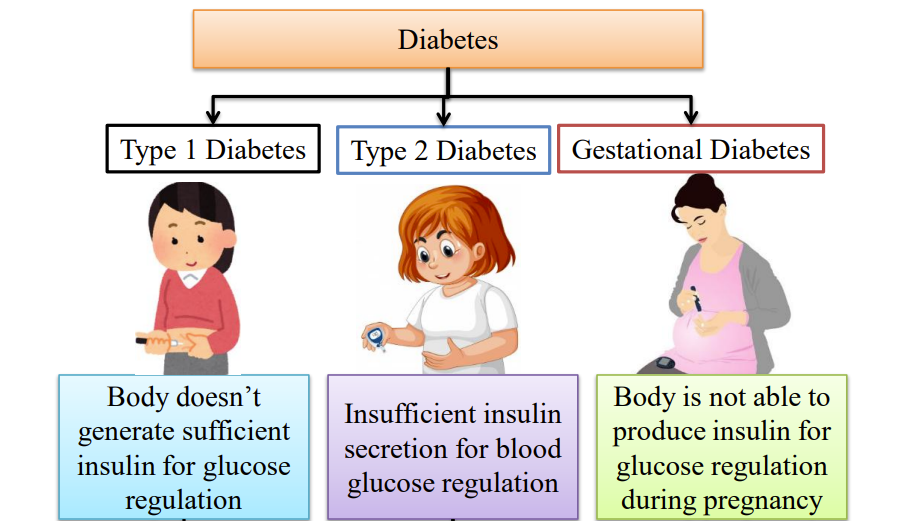
\includegraphics[width=55mm,scale=1.5]{fig/diabetes.png}
            \caption{Types of diabetes.}
            \label{fig:diabetes}
        \end{minipage}
        \hspace{0.5cm}
        \begin{minipage}[b]{0.45\linewidth}
            \centering
            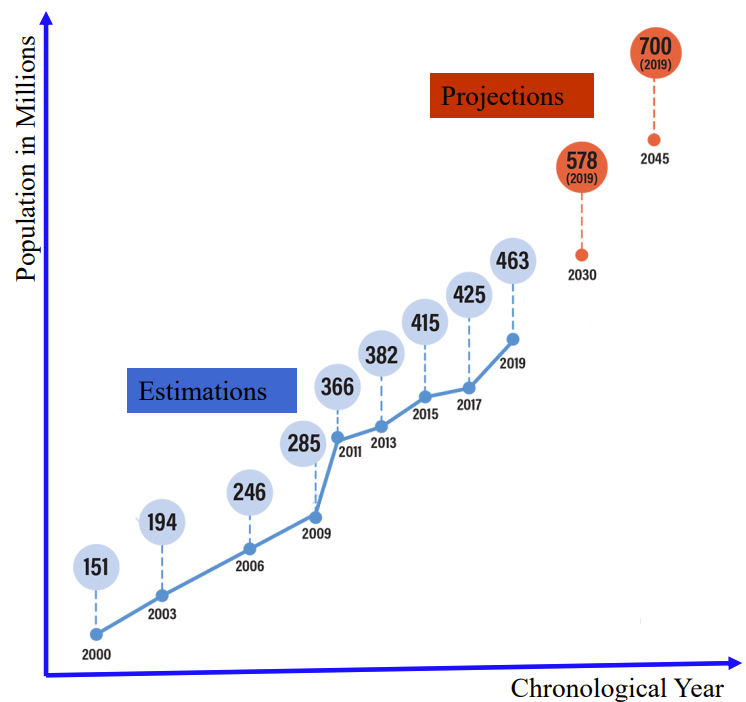
\includegraphics[width=55mm,scale=1.5]{fig/numbers_diabetes.png}
            \caption{Growing numbers of people with diabetes.}
            \label{fig:numbers_diabetes}
        \end{minipage}
    \end{figure}
\end{frame}

\begin{frame}
    \frametitle{Communication System}
    \begin{figure}[H]
        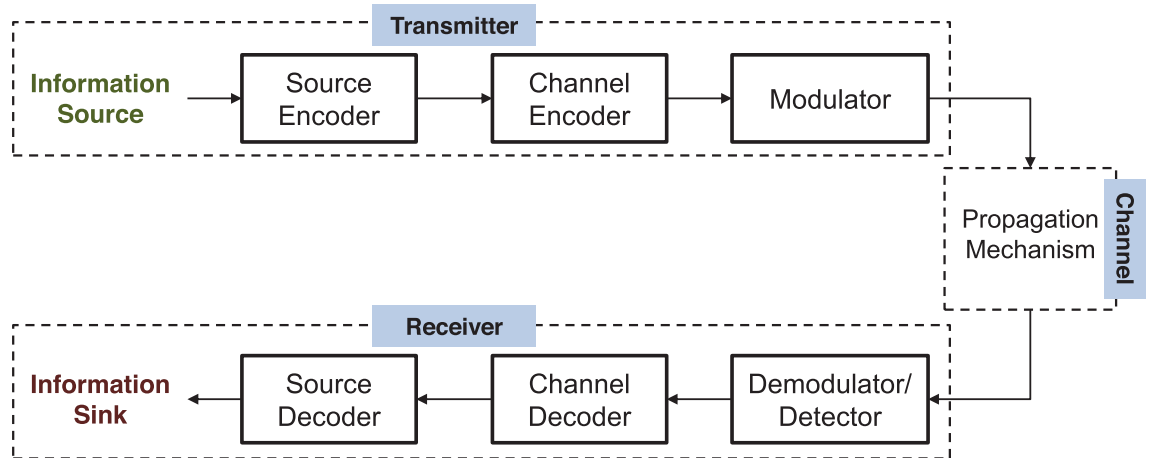
\includegraphics[width=60mm,scale=2]{fig/TC_system.png}
        \caption{Traditional communication system}
    \end{figure}
    \begin{figure}[H]
        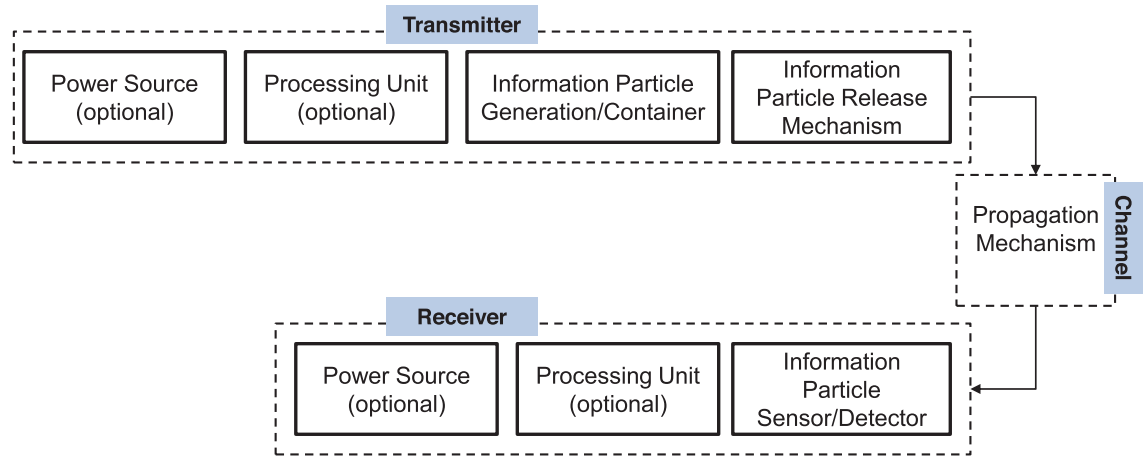
\includegraphics[width=60mm,scale=2]{fig/MC_system.png}
        \caption{Molecular communication system}
    \end{figure}
\end{frame}
\begin{frame}
    \frametitle{Our Research}
    \begin{figure}[h!]
        \centering
        \subfigure[ASK]{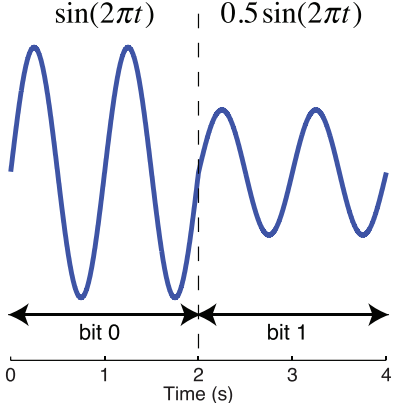
\includegraphics[width=20mm]{fig/ASK.png}}
    \quad 
        \subfigure[FSK]{\includegraphics[width=20mm]{fig/FSK.png}}
    \quad
        \subfigure[PSK]{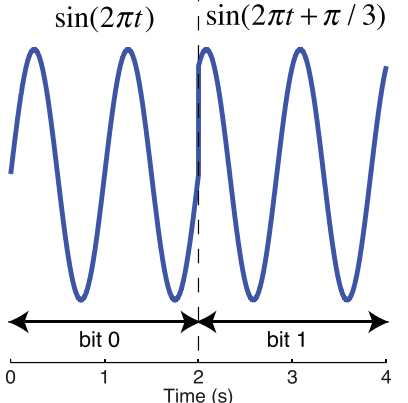
\includegraphics[width=20mm]{fig/PSK.png}}
    \quad
         \subfigure[CSK]{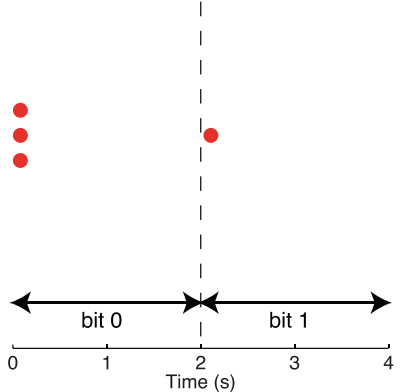
\includegraphics[width=20mm]{fig/CSK.png}}
    \quad 
        \subfigure[MTSK]{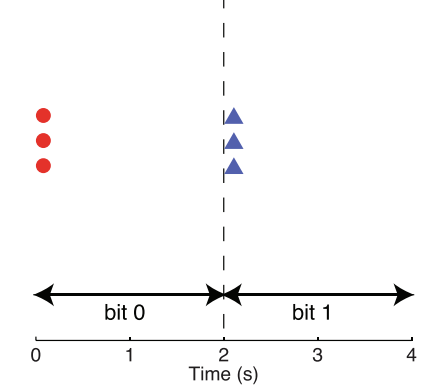
\includegraphics[width=20mm]{fig/MTSK.png}}
    \quad
        \subfigure[RTSK]{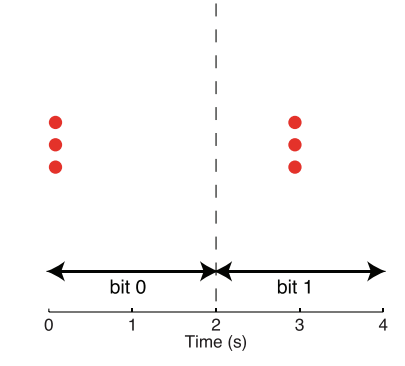
\includegraphics[width=20mm]{fig/RTSK.png}}
        \caption{Different modulation methods}
    \end{figure} 
    \begin{figure}[h!]
        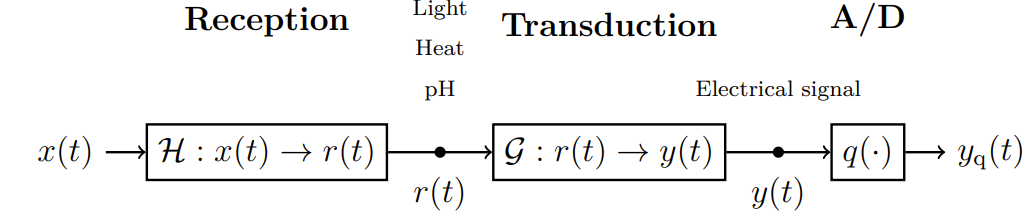
\includegraphics[width=70mm,scale=1]{fig/Research.png}
        \caption{Process at the receiver}
    \end{figure}
    
\end{frame}

\section{Non-invasive: Optical Methods}
\begin{frame}{Theory}
    \begin{columns}[t]
      \begin{column}{.45\textwidth}
        \adjincludegraphics[width= \linewidth, valign=t]{fig/optical_theory.png}
            %\caption{More glucose result in less absorption. }
      \end{column}
      \begin{column}{.5\textwidth}
        \begin{itemize}
          \item Optical reflectometry: intensity of reflected light proportional to GC
          \item Optical transimission: intensity of transmitted light proportional to GC
          
        \end{itemize}
      \end{column}
    \end{columns}
\end{frame}

\begin{frame}{Example of Near Infrared}
    \begin{columns}[t]
        \begin{column}{.45\textwidth}
          \adjincludegraphics[width=70mm, valign=t]{fig/absorbance.png}
        \end{column}
        \begin{column}{.5\textwidth}
          \begin{itemize}
            \item Glucose absorbance value higher than water at wavelength 1500nm-1800nm
            \item Transmittance as measurement method
            \item Transmitted light converted to electric current by photodiode
            \item Beer Lambert Law: \begin{align} I&=I_0e^{-A}\\ A&=k*l*C \end{align}

          \end{itemize}
        \end{column}
    \end{columns}  
    
\end{frame}
\begin{frame}{Implementation}
    \begin{figure}[!htb]\centering
        \begin{minipage}{0.5\textwidth}
          \frame{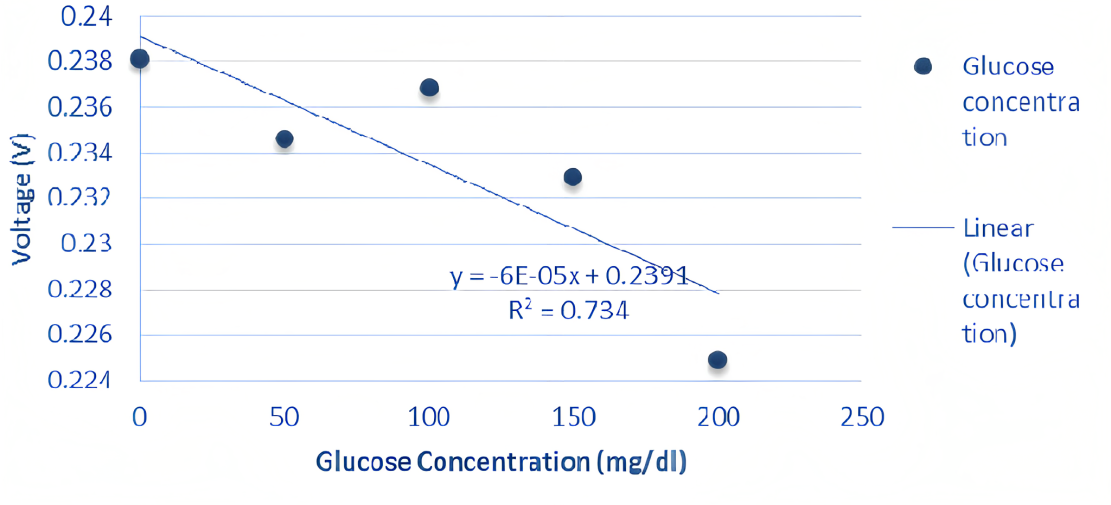
\includegraphics[width=0.9\linewidth]{fig/1550nm.png}}
          \caption{GC-voltage at $\lambda$=1550nm}
        \end{minipage}
        \begin {minipage}{0.48\textwidth}
          \frame{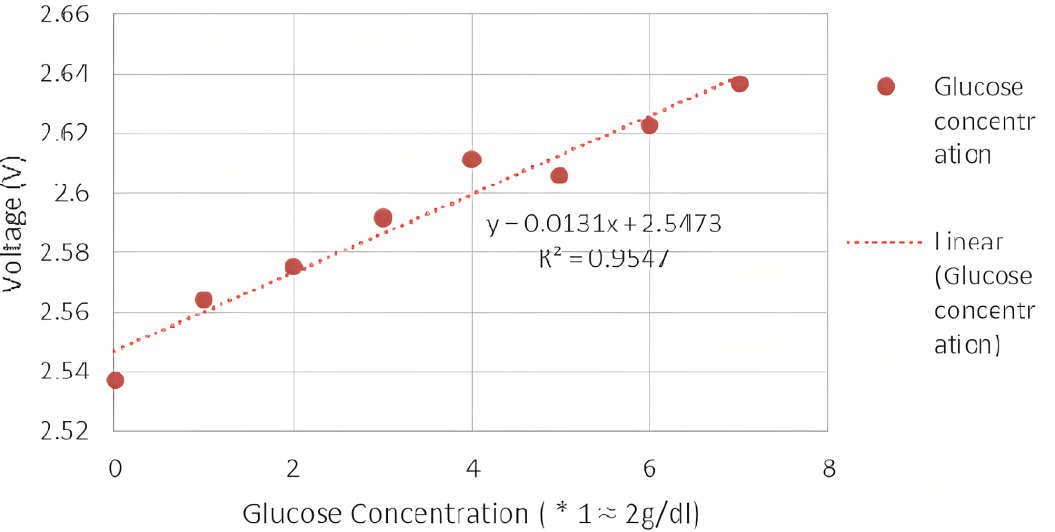
\includegraphics[width=0.9\linewidth]{fig/1300nm.png}}
          \caption{GC-voltage at $\lambda$=1300nm}
        \end{minipage}
     \end{figure}
   \begin{itemize}  
     \item At $\lambda$=1550nm, each 50mg/dl increasing of GC,n3mV raising in photodiode voltage
     \item Increasing GC results in increasing vlotage, means that main absorbent is water
   \end{itemize}
\end{frame}

\begin{frame}{Optical Methods Analysis based on Calrke Erro Grid}
    \begin{table}[htbp]
        \resizebox{\linewidth}{!}{
        \begin{tabular}{|l||c|c|c|} \hline\hline
            
        method & data & advantage & disadvantage\\ \hline
        NIR& A:75\%  B:25\% & intensity is proportional to glucose molecule &high scattering level \\
        MIR &  & glucose molecule absorption stronger & limited penetration \\
        FIR &  A:81\%  B:19\% & frequent calibration is not required &depends on temprature and substance thickness \\
        Occlusion & A:69.7\%  B:25.7\% & enhancement of robustness& \\
        MHC & A:90\%  B:10\% & use well-known various parameters &sensitive to temperature and sweat\\ \hline\hline
        \end{tabular}}
    \end{table}
    \begin{itemize}
        \item MIR with 2500nm-10000nm
        \item FIR with 8000nm-14000nm
        \item Occlusion: pressure applied by using pneumatic cuff to cease blood flow for few seconds
        \item Metabolic heat Conformation: $[GLU]= F(heat generated, blood flow rate, Hb, HbO_2)$
    \end{itemize}
\end{frame}

\begin{frame}
    \begin{figure}[!htb]\centering
        \begin{minipage}{0.5\textwidth}
          \frame{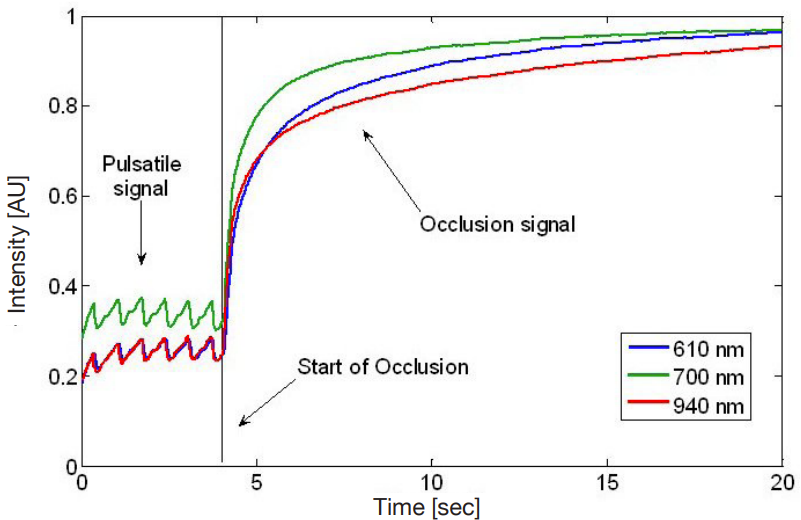
\includegraphics[width=0.9\linewidth]{fig/occlusion.png}}
          \caption{Occlusion signals}
        \end{minipage}
        \begin {minipage}{0.48\textwidth}
          \frame{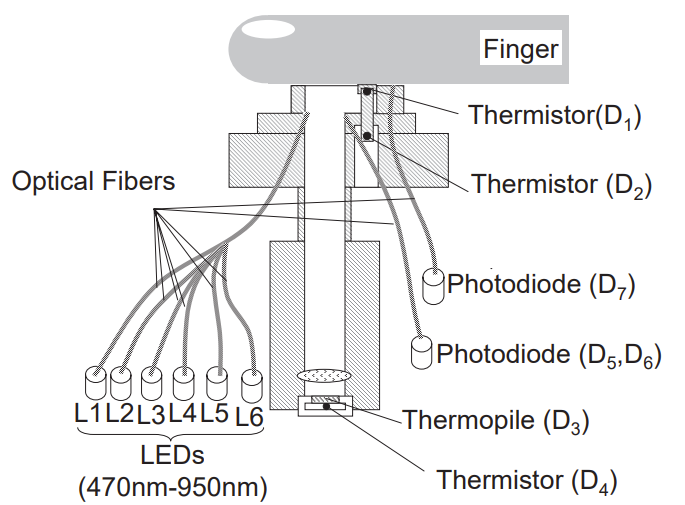
\includegraphics[width=0.9\linewidth]{fig/MHC_device.png}}
          \caption{MHC-deveice}
        \end{minipage}
     \end{figure}
\end{frame}

\begin{frame}
    \begin{figure}[!htb]
        \minipage{0.32\textwidth}
          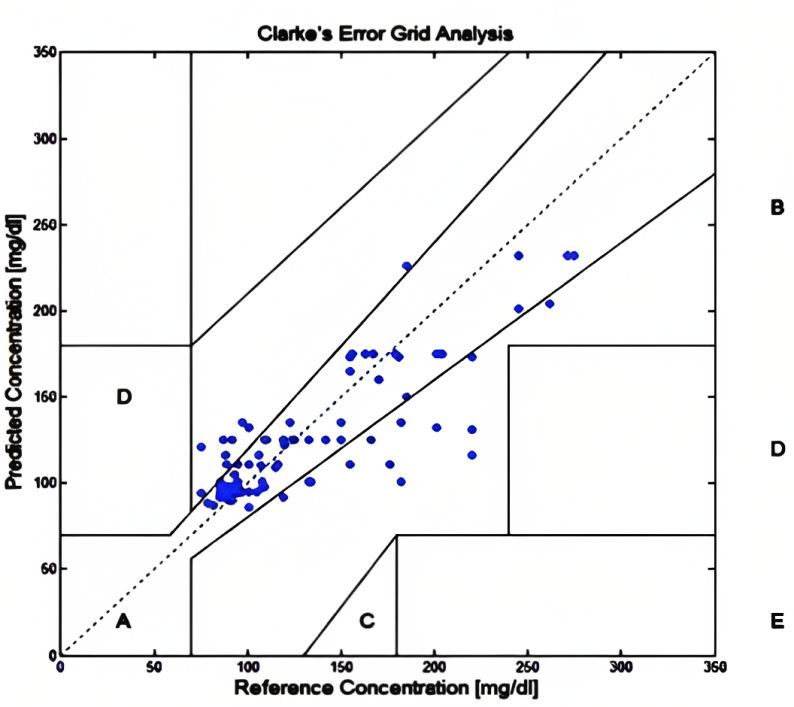
\includegraphics[width=\linewidth]{fig/NIR_ceg.png}
          \caption{NIR-Clarke Erro Grid}
        \endminipage\hfill
        \minipage{0.32\textwidth}
          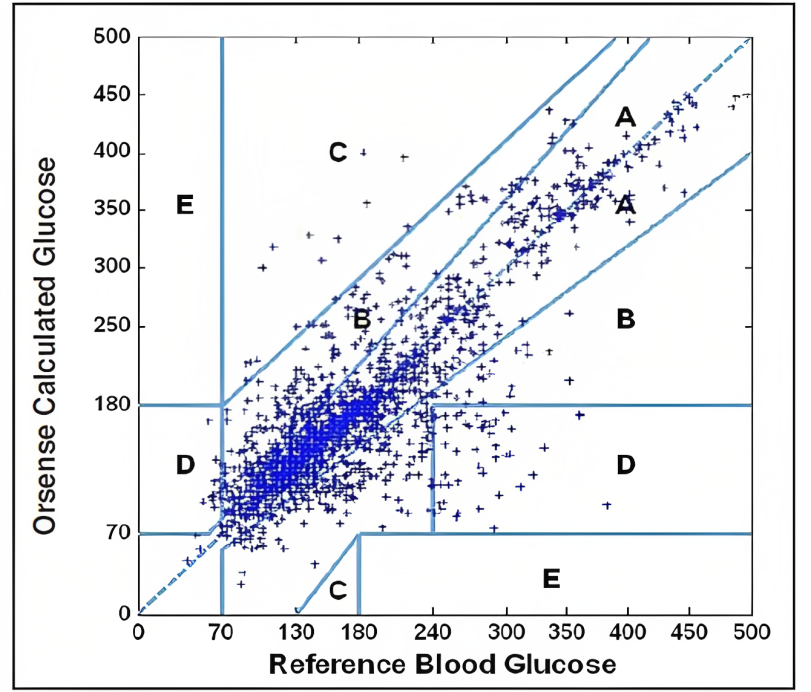
\includegraphics[width=\linewidth]{fig/occlusion_ceg.png}
          \caption{Occlusion-Clarke Erro Grid}
        \endminipage\hfill
        \minipage{0.32\textwidth}%
          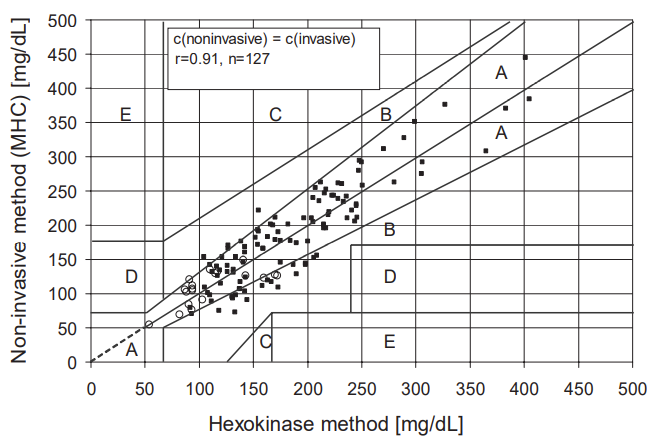
\includegraphics[width=\linewidth]{fig/MHC_ceg.png}
          \caption{MHC-Clarke Erro Grid}
        \endminipage
    \end{figure}
    \begin{itemize}
        \item good performances in real-time, suitable for CCM
        \item effected by fat, protein, water in body
    \end{itemize}
\end{frame}


\section{Enzyme-based: Impedance Spectroscopy}
\begin{frame}{Theory}
    \begin{columns}[t]
        \begin{column}{.45\textwidth}
          \adjincludegraphics[width= \linewidth, valign=t]{fig/ATP.png}
              %\caption{More glucose result in less absorption. }
        \end{column}
        \begin{column}{.5\textwidth}
          \begin{itemize}
            \item Glucose converted to ATP
            \item ATP controls ion pump channel 
            \item Ion permitivity of cell membrane changes
            \item Detected by field-effect transistor
          \end{itemize}
        \end{column}
    \end{columns}
\end{frame}
\begin{frame}{Model of Impedance Spectroscopy}
    \begin{figure}[h!]
        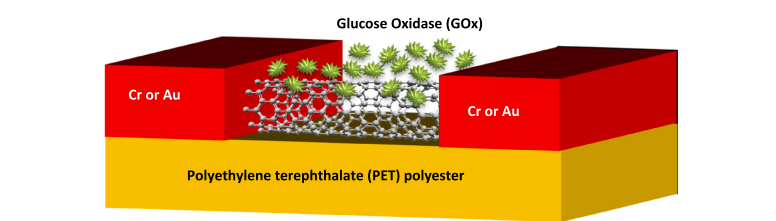
\includegraphics[width=\textwidth]{fig/SWCNT.png}
        \caption{Proposed combination of metal electrodes, a layer of $GO_x$ biomolecular assembl, and SWCNT Channel in FET}
    \end{figure}
\end{frame}

 
        
\begin{frame}
  \begin{figure}[h!]
    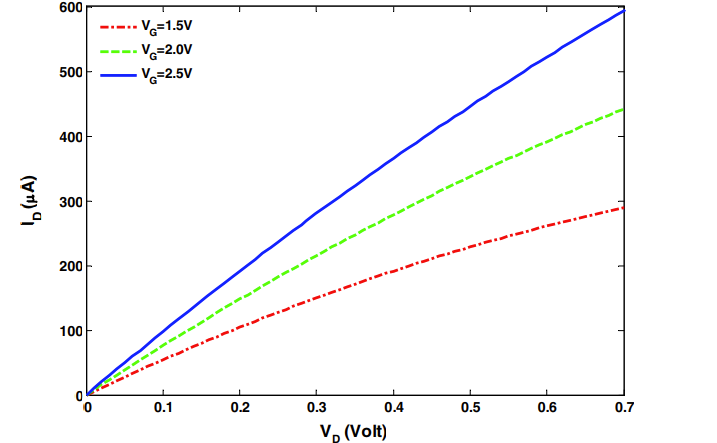
\includegraphics[width=0.4\linewidth,scale=0.4]{fig/bare_SWCNT.png}
    \caption{Comprehensive glucose sensing mechanism}
    \begin{itemize}
      \item  Bare transistor: \begin{equation} I_D=\beta(2V_{GT}V_D-V_{D}^2)/(1+V_D/V_c) \end{equation}
      \item  Transistor with solution:\begin{align}
        V_{GT1}= V_{GT} + V_{PBS}-V_{T}\\
        I_D=[2(V_{GT1}V_D)-V_{D}^2]/(1+V_D/V_c)
      \end{align}
    \end{itemize}
    
        
  \end{figure}
\end{frame}     
  

\begin{frame}
  \begin{figure}[h!]
    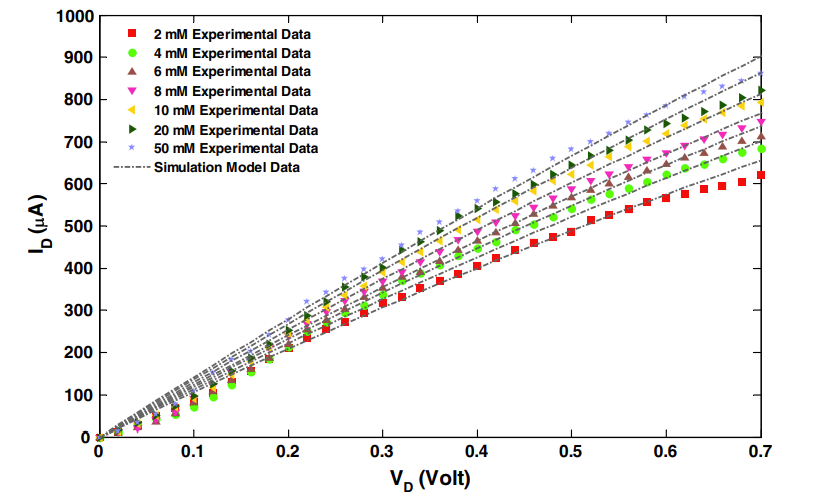
\includegraphics[width=0.4\linewidth,scale=0.4]{fig/glucose_SWCNT.png}
    \caption{Comprehensive glucose sensing mechanism}
    \begin{itemize}
      \item Transistor with glucose:\begin{equation}
      I_D=[2(V_{GT1}+V_{glucose})V_D-V_D^2]/(1+V_D/V_c)\end{equation}
      \item Glucose concentration against gate voltage:\begin{equation}
      V_{glucose}(C)= 1.42 V-\exp{(-0.1C)}\end{equation}
      \item Drain current to glucose concentration:\begin{equation}
      I_D=[2(V_{GT1}+1.42 V-\exp{(-0.1C)})V_D-V_D^2]/(1+V_D/V_c)\end{equation}
    \end{itemize}
  \end{figure}
\end{frame}

\begin{frame}
  \begin{figure}[h!]
    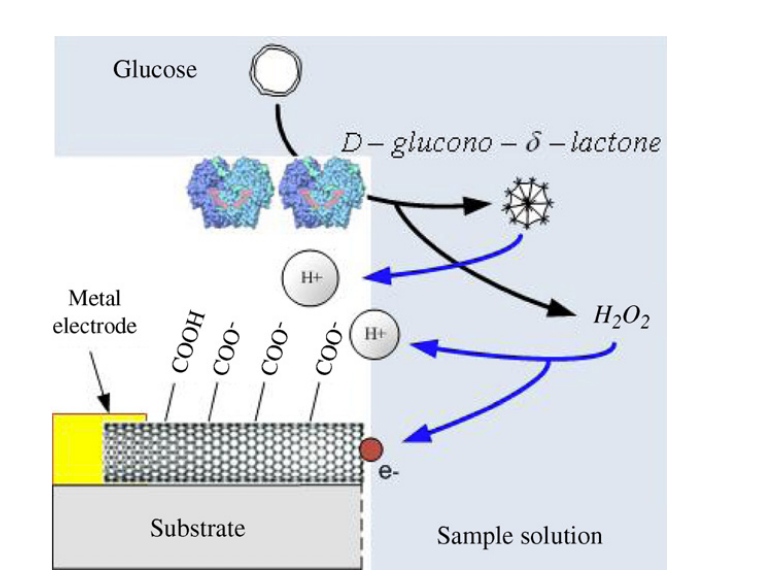
\includegraphics[width=0.3\linewidth,scale=0.3]{fig/reaction_FET.png}
    \caption{Comprehensive glucose sensing mechanism}
    \begin{itemize}
      \item  Involved reactions:
      \begin{align}
        \ch{
          O2 +  $\beta$-D-Glucose &->[GOx] H2O2 + D-glucose-$\beta$-lactone  \label{Oxygen}\\
          H2O + D-glucose-$\beta$&-lactone     -> H+ + D-gluconate^- \label{glucose}\\
          H2O2 &->[0.7V] O2 + 2 H+ + 2 e^- \label{FADH}
          }
    \end{align}
      \end{itemize}
  \end{figure}
\end{frame}

\begin{frame}{Analysis of results}
  \begin{columns}[t]
    \begin{column}{.4\textwidth}
      \adjincludegraphics[width=\linewidth, valign=t]{fig/limitation_rate.png}
      \begin{equation}
        \ch{E + S <=>[k 1][k 3] ES ->[k 2] E + P} 
        \label{eq:MMK}
    \end{equation}
    \end{column}
    \begin{column}{.5\textwidth}
      \begin{itemize}
        \item  Michaelis-Menten kinetics:
        
        \begin{align}
          \frac{\mathrm{d}[E]}{dt}&= (k_2+k_3)[ES]-k_1[E][S] \\
          \frac{\mathrm{d}[S]}{dt}&= k_3[ES]-k_1[E][S] \\
          \frac{\mathrm{d}[ES]}{dt}&= k_1[E][S]-(k_2+k_{3})[ES] \\
          \frac{\mathrm{d}[P]}{dt}&= k_2[ES]
          %\frac{\mathrm{d}[P]}{dt} = \frac{k_2[E]_0\cdot [S]}{\frac{k_{3}+k_2}{k_1}+[S]}
        \end{align} 
    \end{itemize}
  \end{column}
  \end{columns}
\end{frame}

\begin{frame}{Simulation}
 
\end{frame}
\section{Enzyme-based: Electrochemistry Method}
\begin{frame}{Theory}
  \begin{figure}[h!]
    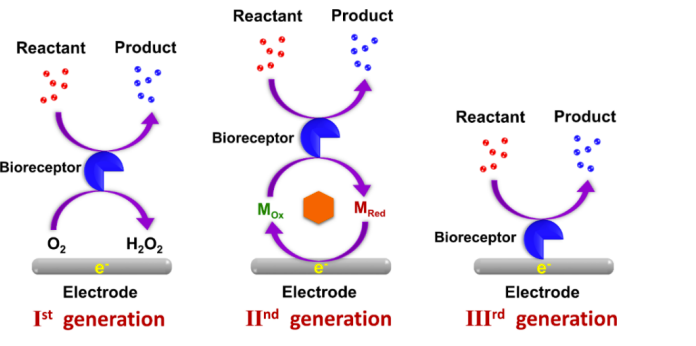
\includegraphics[width=0.5\textwidth,scale=.5]{fig/biosensor_123generation.png}
    \begin{itemize}
      \item 1st-generation: GOx-catalyzed oxidation of glucose, measure generated $H_2O_2$ by the enzyme or the consume of $O_2$
      \item 2nd-generation:$O_2$ replaced, a sythetic electron recipient 
      \item 3rd-generation: direct electron transfer (DET)
    \end{itemize}
  \end{figure}
\end{frame}

\begin{frame}{Model of Electrochemistry Biosensor}
  \begin{figure}[h!]
    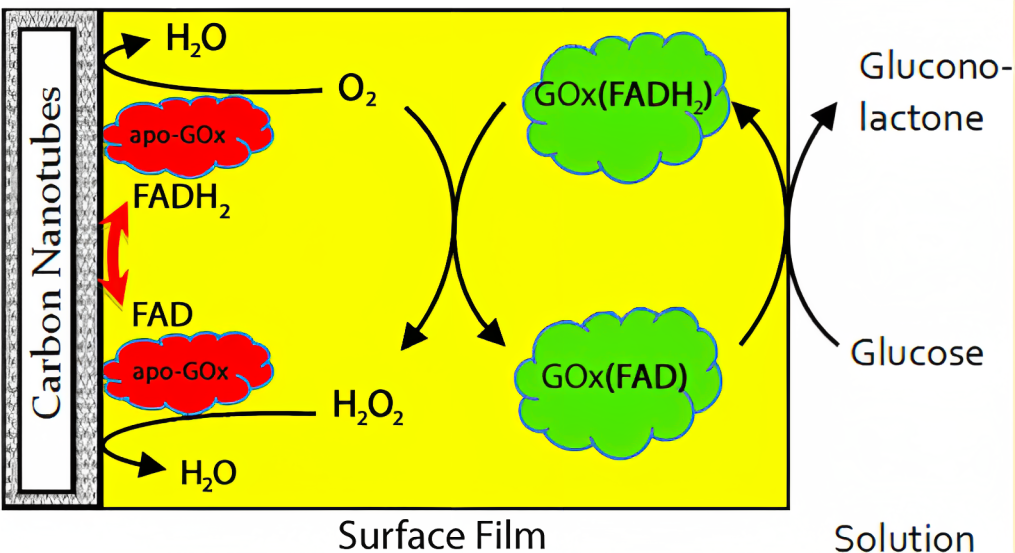
\includegraphics[width=0.4\textwidth,scale=.2]{fig/biochemical_sensor.png}
    \begin{itemize}
      \item Involved reactions:
      \begin{align}
        \ch{
          O2 + 4 H+ + 4 e^-(CNT) &-> H2O2 + 2 H+ + 2 e^-(CNT) -> 2 H2O \\
          GOx(FAD)^{CNT} + $\beta$-D-Glucose  &-> GOx(FADH2)^{CNT} + D-glucose - 1,5 -lactone \\
          GOx(FADH2)^{CNT} + O2 &-> GOx(FAD)^{CNT} + H2O2 \\
          FAD + 2 H+ + 2 e^- &<-> FADH2 
          }
       \end{align}
    \end{itemize}
  \end{figure}
\end{frame}

\begin{frame}{Analysis of Model}
  \begin{figure}[h!]
    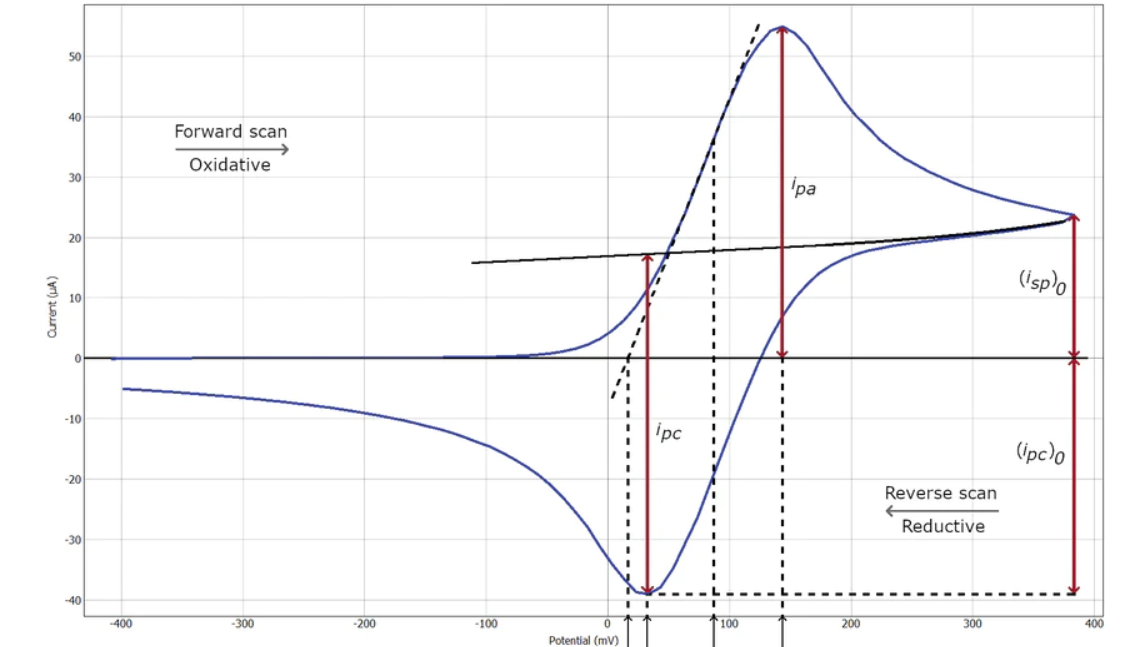
\includegraphics[width=0.4\textwidth,scale=.2]{fig/CV.png}
    \caption{Cyclic voltammetry}
    \begin{itemize}
      \item  Investigate the reduction and oxidation processes of molecular species
      \item  Peak potential and peak current:  \begin{align}
        \delta E_p &= E_{pa}-E_{pc} =0.059/n\\   
        i_p &=(2.69 \times 10^5)n^{3/2}SD^{1/2}Cv^{1/2}  \label{i_p}
        \end{align}
    \end{itemize}
\end{figure}
\end{frame}


\begin{frame}
  \begin{figure}[h!]
    \centering
    
       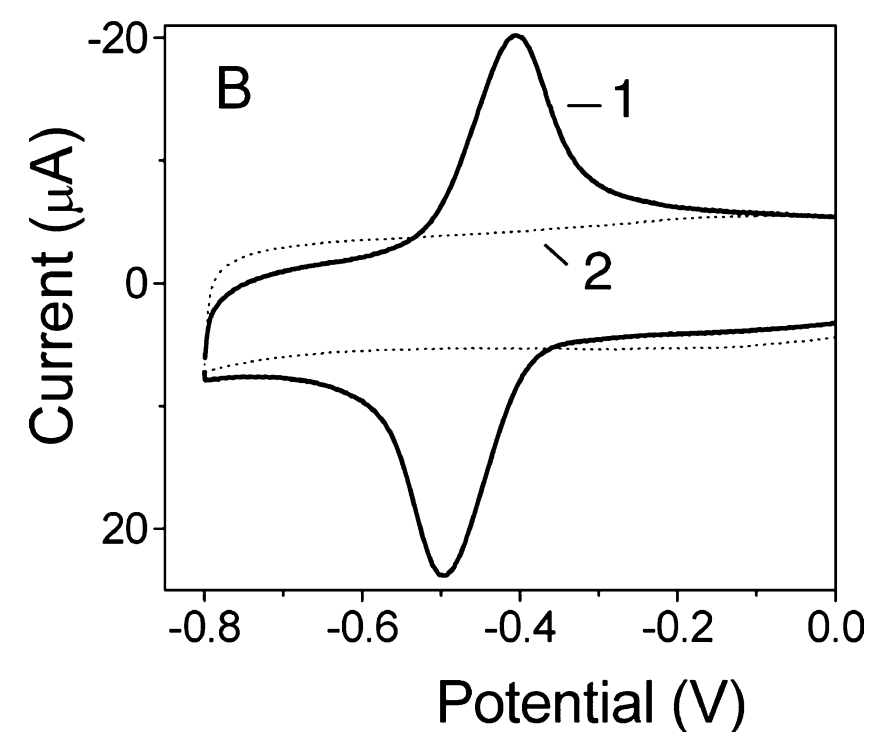
\includegraphics[width=0.4\textwidth]{fig/FAD.png}
       \caption{CV of FAD}
    \end{figure}
    \begin{itemize}
      \item $O_2$-free solutions: exist a pair of peaks
      
    \end{itemize}
\end{frame}
\begin{frame}
  \begin{figure}[h!]
    \centering
    
       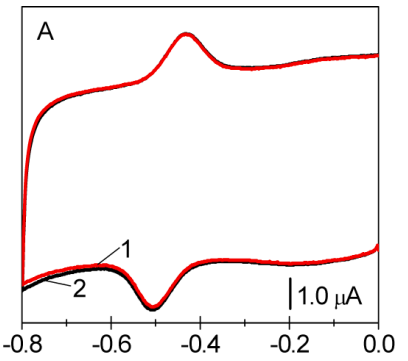
\includegraphics[width=0.4\textwidth]{fig/FADwithglucose.png}
       \caption{CV of FAD}
    \end{figure}
    \begin{itemize}
      \item Glucose added into $O_2$-free solution: not effect the
      result of the electroactivity 
      
    \end{itemize}
\end{frame}

\begin{frame}
  \begin{figure}[h!]
    \centering
    
       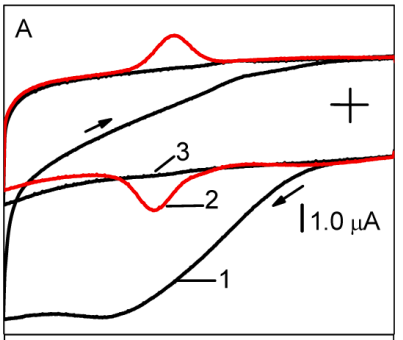
\includegraphics[width=0.4\textwidth]{fig/oxygewithfad.png}
       \caption{CV of FAD}
    \end{figure}
    \begin{itemize}
      \item $O_2$-containing solutions with only FAD
     \end{itemize}
\end{frame}


\begin{frame}
  \begin{figure}[h!]
    \centering
    
       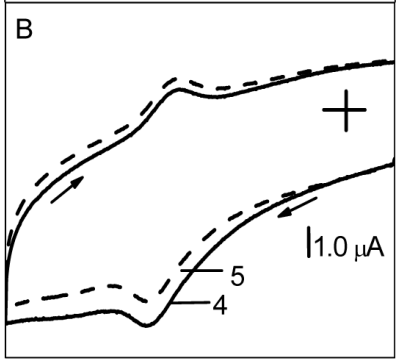
\includegraphics[width=0.4\textwidth]{fig/solutionwithglucose.png}
       \caption{CV of FAD}
    \end{figure}
    \begin{itemize}
      \item $O_2$-containing solutions also with glucose: electrochemical peak current of Oxygen decrease
     \end{itemize}
\end{frame}
\begin{frame}
  \begin{itemize}
    \item assumption:
 
  \begin{equation} 
    i_{ptotal} =(2.69 \times 10^5)n^{3/2}SD^{1/2}C_{O_2}v^{1/2} + i_{FAD}
    \end{equation}
    %Due to glucose has no effect on the produced current of FAD, we can use differential analysis to eliminate the interference. Then we assume another same solution with glucose now.Enzyme,e,g.FAD accelerates the reaction of Glucose with velocity $V_a$, it should be $k$ proportional to $\log C_{glucose}$. We can get the produced velocity of $FADH_2$, which correspondingly shows $V_{O_2consumed}$, e.g., the consume velocity of Oxygen. Now the part of Oxygen, which undergoes electrochemistry will be calculated as the following: 
    \begin{equation}
       C_{O_2electro}= C_{O_2}- v_{O_2consumed}= C_{O_2} - k \times log C_{glucose}
    \end{equation}
    %The peak current of Oxygen with glucose in the solution represents as $i_{pnew}$, which equals to:
    \begin{equation}
       i_{pnew} = (2.69 \times 10^5)n^{3/2}SD^{1/2}C_{O_2electro}v^{1/2} + i_{FAD}
    \end{equation}
    %At last we can derive formula between glucose concentration $C_{glucose}$ and differential peak current $\delta i_{p}$ as below: 
    \begin{equation}
       \delta i_{p} = (2.69 \times 10^5)n^{3/2}SD^{1/2} (C_{O_2} - k \times log C_{glucose})v^{1/2}
    \end{equation}
  \end{itemize}
\end{frame}
\section{Conclusions}
\begin{frame}{Conclusions}
  \begin{itemize}
    \item [$\blacktriangleright$] Optical methods: change in the refractive index, light absorption, or
    fluorescence of glucose
        \begin{itemize}
          \item Detecting glucose changes in real-time
          \item Sensitive to other components in the body
        \end{itemize}

    \item [$\blacktriangleright$]Enzyme-based methods:
        \begin{itemize}
        \item Impedance spectroscopy: change of impedance proportional to GC 
        \item Electrochemistry: electrical signal generated by the oxidation of glucose directly measured 
        \item High-precision
        \item Instability due to enzyme, susceptible to denaturation and inactivation over time 
        
    \end{itemize}
    \item [$\blacktriangleright$]Further work: evaluation of the reconstruction accuracy for molecule concentration signals (pulse position modulated signals, concentration shift keying modulated
    signals, etc., for receivers with fixed operators
  \end{itemize}
   \
\end{frame}
 

\begin{frame}
\centering
\vspace{.3\textheight}
\huge Thank You for Your Attention!\\
\pause
\vspace{1cm}
\huge Questions?
\end{frame}


\end{document}
